\documentclass[12pt,a4paper]{article}

% ============================================================
% PACKAGES
% ============================================================
\usepackage[a4paper,margin=1in]{geometry}
\usepackage{graphicx}
\usepackage{float}
\usepackage{placeins}
\usepackage{tabularx}
\usepackage{array}
\usepackage{booktabs}
\usepackage{longtable}
\usepackage{enumitem}
\usepackage{xcolor}
\usepackage{hyperref}
\usepackage{setspace}
\usepackage{fancyhdr}
\usepackage{titlesec}
\usepackage{needspace}
\usepackage{caption}

% ============================================================
% COLORS
% ============================================================
\definecolor{linkblue}{RGB}{0,90,170}

% ============================================================
% HYPERLINK SETTINGS
% ============================================================
\hypersetup{
    colorlinks=true,
    linkcolor=linkblue,
    urlcolor=linkblue,
    citecolor=linkblue,
    pdftitle={InternNova Week 3 - Malware, Phishing & Security Awareness},
    pdfauthor={NAJMUDEEN S}
}

% ============================================================
% DOCUMENT SETTINGS
% ============================================================
\setstretch{1.08}
\setlength{\parindent}{0pt}
\setlength{\parskip}{6pt}
\setlist[itemize]{leftmargin=1.5em}
\setlist[enumerate]{leftmargin=1.7em}
\setlength{\emergencystretch}{3em}
\sloppy
\urlstyle{same}
\Urlmuskip=0mu plus 1mu

% ============================================================
% HEADING FORMATTING
% ============================================================
\titleformat{\section}{\Large\bfseries}{\thesection}{0.7em}{}
\titleformat{\subsection}{\large\bfseries}{\thesubsection}{0.7em}{}
\titleformat{\subsubsection}{\normalsize\bfseries}{\thesubsubsection}{0.7em}{}

% ============================================================
% HEADER AND FOOTER
% ============================================================
\pagestyle{fancy}
\fancyhf{}
\fancyhead[L]{\small\textbf{InternNova -- Week 3}}
\fancyhead[R]{\small\textbf{Malware, Phishing \& Security Awareness}}
\fancyfoot[C]{\thepage}
\renewcommand{\headrulewidth}{0.4pt}
\renewcommand{\footrulewidth}{0pt}
\setlength{\headheight}{15pt}

% ============================================================
% REFERENCE COMMANDS FROM THE ORIGINAL TASK FILES
% ============================================================
\newcommand{\refs}[3]{%
    \textbf{Reference Basis:} Authoritative cybersecurity guidance\par
    \textbf{Reference Paper / Standard:} Relevant guidance or standard\par
    \textbf{Learning Video:} Educational cybersecurity video\par
    \href{#1}{\textcolor{linkblue}{View Reference}}
    \quad
    \href{#2}{\textcolor{linkblue}{View Standard}}
    \quad
    \href{#3}{\textcolor{linkblue}{Watch on YouTube}}
}

\newcommand{\referenceblock}[2]{%
\begin{samepage}
\noindent\textbf{Reference basis:} #1\par
\smallskip
\noindent\url{#2}\par
\end{samepage}
\par\vspace{0.25cm}
}

\newcommand{\paperblock}[2]{%
\begin{samepage}
\noindent\textbf{Reference / Standard:} #1\par
\smallskip
\noindent\url{#2}\par
\end{samepage}
\par\vspace{0.25cm}
}

\newcommand{\videoblock}[3]{%
\begin{samepage}
\noindent\textbf{Learning Video -- S.No. #1:} #2\par
\smallskip
\noindent\url{#3}\par
\end{samepage}
\par\vspace{0.25cm}
}

% ============================================================
% TABLE OF CONTENTS FORMATTING
% ============================================================
\setcounter{tocdepth}{2}
\renewcommand{\contentsname}{Table of Contents}

\begin{document}

% ============================================================
% MAIN COVER PAGE — UNNUMBERED
% ============================================================
\pagenumbering{gobble}
\pagestyle{empty}
% ============================================================
% COVER PAGE
% ============================================================


% ---------- Cover ----------
\begin{titlepage}
\centering
\vspace*{1.5cm}

{\Large\textbf{InternNova Internship Program}\par}
\vspace{0.8cm}

{\large\textbf{Week 3 Assignment}\par}
\vspace{1.2cm}

{\LARGE\textbf{Malware, Phishing \& Security Awareness}\par}
\vspace{1.0cm}

{\Large\textbf{Task 1 \& Task 2}\par}
\vspace{0.6cm}

{\large\textbf{Malware, Phishing \& Security Awareness}\par}

\vfill

\begin{tabular}{>{\bfseries}l l}
Intern Name: & NAJMUDEEN S\\
Internship: & InternNova\\
Week: & 3\\
Assignment: & Malware, Phishing \& Security Awareness\\
Month: & October 2026\\
\end{tabular}

\vfill

\end{titlepage}

% ============================================================
% TABLE OF CONTENTS — UNNUMBERED
% ============================================================
\clearpage
\thispagestyle{empty}
\tableofcontents

% ============================================================
% MAIN CONTENT — PAGE 1 STARTS HERE
% ============================================================
\clearpage
\pagenumbering{arabic}
\setcounter{page}{1}
\pagestyle{fancy}

% ============================================================
% TASK 1
% ============================================================

\section{Task 1: Understanding Malware}

\subsection{Introduction}

Malware is short for malicious software. It refers to software designed to perform unauthorized or harmful actions on a computer, mobile device, network, or information system. Different malware types behave differently: some infect files, some spread between systems, some disguise themselves as legitimate software, some restrict access to data, and some secretly collect information.

% ============================================================
% VIRUS
% ============================================================

\subsection{Virus}

\subsubsection{Definition}

A virus is malware that attaches itself to a file or program and can replicate when the infected content is executed.

\subsubsection{How It Works}

A typical virus becomes active when an infected file is executed. The malicious code can then modify or attach itself to other files, allowing the infection to continue when those files are opened or shared.

\begin{figure}[H]
\centering
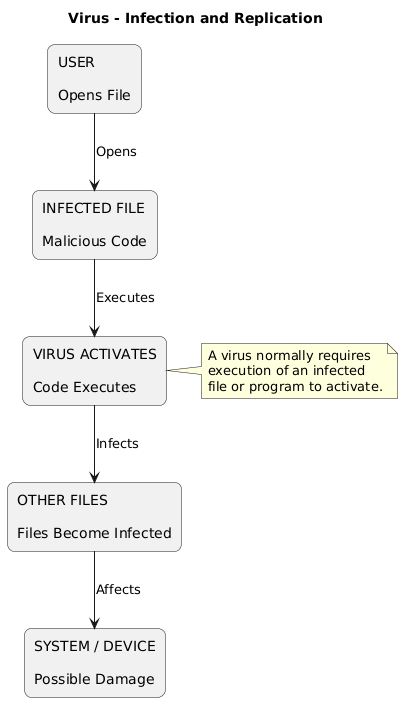
\includegraphics[width=.58\textwidth]{images/virus.png}
\caption{Virus Infection and Replication}
\end{figure}

\subsubsection{Real-World Example}

CIH, also known as the Chernobyl virus, is a historical example of a computer virus associated with infected executable files and destructive activity.

\subsubsection{Cybersecurity Connection}

Viruses are relevant to endpoint security because they can modify legitimate files and affect system integrity. Analysts may investigate antivirus detections, unusual file modifications, suspicious processes, and unexpected system behavior.

\subsubsection{Security Risk and Protection}

\textbf{Potential Risk:} An infected file can spread malicious code when it is executed or shared.

\textbf{Protection:}

\begin{itemize}
    \item Use reputable security software.
    \item Keep systems updated.
    \item Avoid unexpected attachments.
    \item Download software from trusted sources.
    \item Scan suspicious files.
\end{itemize}

\refs
{https://www.cisa.gov/news-events/news/malware}
{https://www.cisa.gov/news-events/news/malware}
{https://www.youtube.com/results?search_query=Professor+Messer+malware+virus}

% ============================================================
% WORM
% ============================================================

\subsection{Worm}

\subsubsection{Definition}

A worm is malware that can replicate itself and spread from one system to another without requiring the user to manually copy it.

\subsubsection{How It Works}

A worm may search for reachable or vulnerable systems and attempt to spread automatically. An infected system can then continue the propagation process.

\begin{figure}[H]
\centering
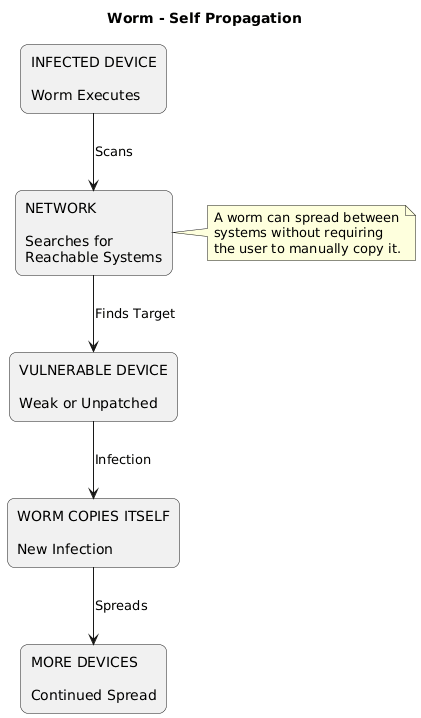
\includegraphics[width=.58\textwidth]{images/worm.png}
\caption{Worm Self-Propagation}
\end{figure}

\subsubsection{Real-World Example}

Conficker is a well-known computer worm that spread through Windows systems by exploiting vulnerabilities and weak configurations.

\subsubsection{Cybersecurity Connection}

Worms are important in network security because they can spread rapidly. Analysts may monitor unusual network traffic, repeated connection attempts, vulnerability exploitation, and unexpected endpoint behavior.

\subsubsection{Security Risk and Protection}

\textbf{Potential Risk:} A worm can automatically spread across vulnerable systems.

\textbf{Protection:}

\begin{itemize}
    \item Apply security updates.
    \item Use firewalls.
    \item Disable unnecessary services.
    \item Segment networks where appropriate.
    \item Monitor unusual network activity.
\end{itemize}

\refs
{https://www.cisa.gov/news-events/news/malware}
{https://www.cisa.gov/news-events/news/malware}
{https://www.youtube.com/results?search_query=Professor+Messer+computer+worm+malware}

% ============================================================
% TROJAN
% ============================================================

\subsection{Trojan}

\subsubsection{Definition}

A Trojan is malware that disguises itself as legitimate or useful software to trick a user into installing or executing it.

\subsubsection{How It Works}

A Trojan may be distributed through a fake application, document, attachment, or apparently legitimate file. After execution, it can perform unauthorized actions.

\begin{figure}[H]
\centering
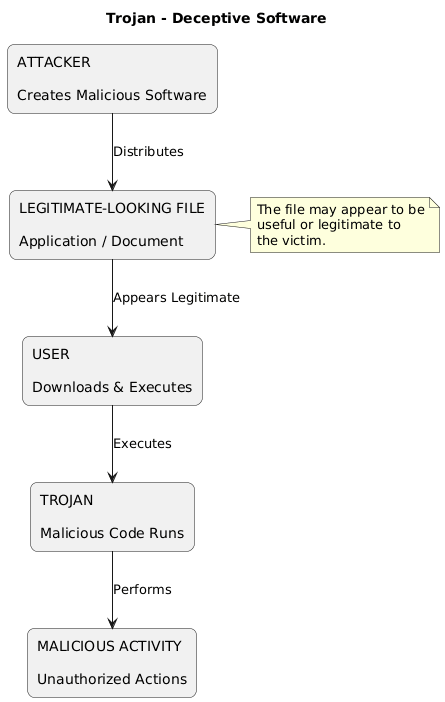
\includegraphics[width=.58\textwidth]{images/trojan.png}
\caption{Trojan Deceptive Software Process}
\end{figure}

\subsubsection{Real-World Example}

Zeus is a well-known example of malware associated with Trojan-based distribution and theft of sensitive information such as banking credentials.

\subsubsection{Cybersecurity Connection}

Trojans are important because they often depend on deception or social engineering. Analysts may investigate unexpected installations, suspicious processes, unusual connections, and endpoint alerts.

\subsubsection{Security Risk and Protection}

\textbf{Potential Risk:} A user may unknowingly install malicious software because it appears legitimate.

\textbf{Protection:}

\begin{itemize}
    \item Use trusted software sources.
    \item Avoid pirated or modified software.
    \item Verify software publishers.
    \item Use endpoint security.
    \item Avoid unexpected attachments.
\end{itemize}

\refs
{https://www.cisa.gov/news-events/news/malware}
{https://www.cisa.gov/news-events/news/malware}
{https://www.youtube.com/results?search_query=Professor+Messer+Trojan+malware}

% ============================================================
% RANSOMWARE
% ============================================================

\subsection{Ransomware}

\subsubsection{Definition}

Ransomware is malware that can prevent access to files or systems, commonly by encrypting data, and then demands payment from the victim.

\subsubsection{How It Works}

Ransomware may enter through a malicious attachment, compromised account, vulnerable service, or another initial access method. It may identify files, encrypt them, and display a ransom demand.

\begin{figure}[H]
\centering
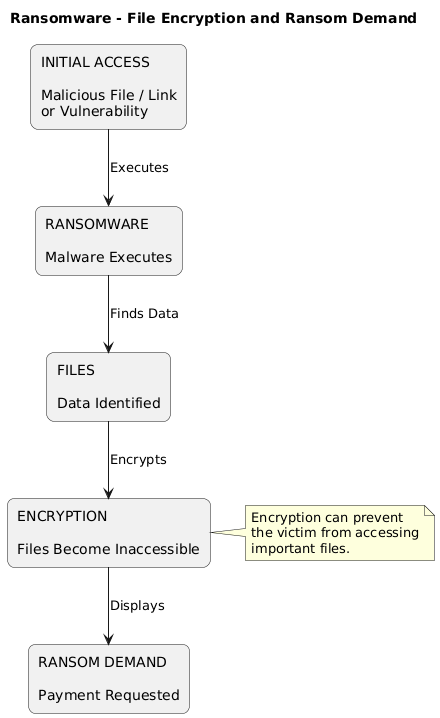
\includegraphics[width=.58\textwidth]{images/ransomware.png}
\caption{Ransomware File Encryption and Ransom Demand}
\end{figure}

\subsubsection{Real-World Example}

WannaCry is a well-known ransomware outbreak that affected computer systems in multiple countries.

\subsubsection{Cybersecurity Connection}

Ransomware can affect data availability and operations. Security teams may monitor endpoint alerts, file activity, authentication events, backups, and network traffic.

\subsubsection{Security Risk and Protection}

\textbf{Potential Risk:} Important files may become inaccessible and operations may be disrupted.

\textbf{Protection:}

\begin{itemize}
    \item Maintain protected backups.
    \item Patch systems.
    \item Use endpoint security.
    \item Restrict unnecessary network access.
    \item Train users to recognize suspicious links and attachments.
\end{itemize}

\refs
{https://www.cisa.gov/stopransomware}
{https://www.cisa.gov/stopransomware/ransomware-guide}
{https://www.youtube.com/results?search_query=Professor+Messer+ransomware}

% ============================================================
% SPYWARE
% ============================================================

\subsection{Spyware}

\subsubsection{Definition}

Spyware is malware designed to operate without the user's knowledge and collect information about user activity or sensitive information.

\subsubsection{How It Works}

Spyware may run in the background after installation. Depending on its capabilities, it can collect browsing activity, credentials, or other sensitive data and transmit it to an unauthorized party.

\begin{figure}[H]
\centering
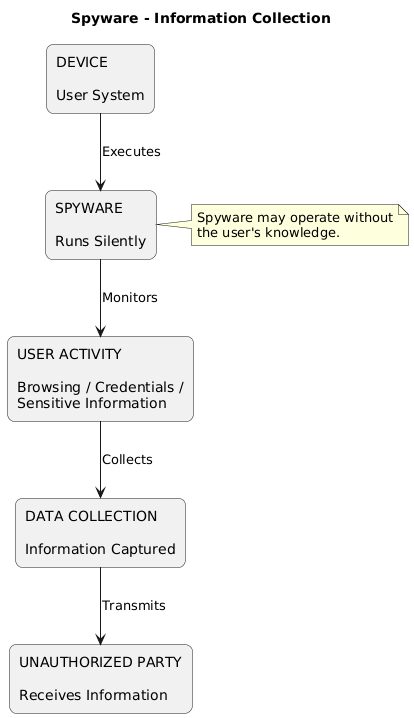
\includegraphics[width=.58\textwidth]{images/spyware.png}
\caption{Spyware Information Collection}
\end{figure}

\subsubsection{Real-World Example}

Pegasus is an example of sophisticated spyware associated with targeted surveillance of mobile devices.

\subsubsection{Cybersecurity Connection}

Spyware is relevant to endpoint security and privacy because unauthorized collection can expose sensitive data. Analysts may investigate unusual processes, applications, connections, and endpoint alerts.

\subsubsection{Security Risk and Protection}

\textbf{Potential Risk:} Sensitive information may be collected without the user's knowledge.

\textbf{Protection:}

\begin{itemize}
    \item Install trusted applications.
    \item Keep systems updated.
    \item Use reputable security software.
    \item Review applications and permissions.
    \item Avoid suspicious links and downloads.
\end{itemize}

\refs
{https://www.cisa.gov/news-events/news/malware}
{https://www.cisa.gov/news-events/news/malware}
{https://www.youtube.com/results?search_query=Professor+Messer+spyware+malware}

% ============================================================
% OVERALL MALWARE DIAGRAMS
% ============================================================


\subsection{Overall Malware Diagrams}

\begin{figure}[H]
\centering
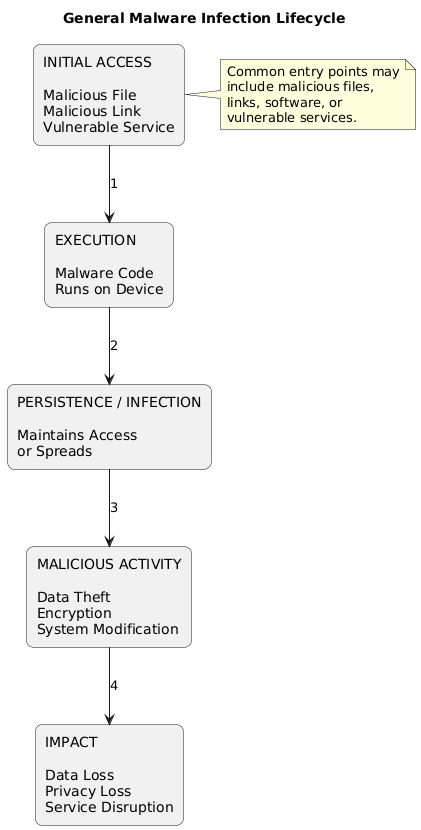
\includegraphics[width=.68\textwidth]{images/malware_lifecycle.png}
\caption{General Malware Infection Lifecycle}
\end{figure}

\begin{figure}[H]
\centering
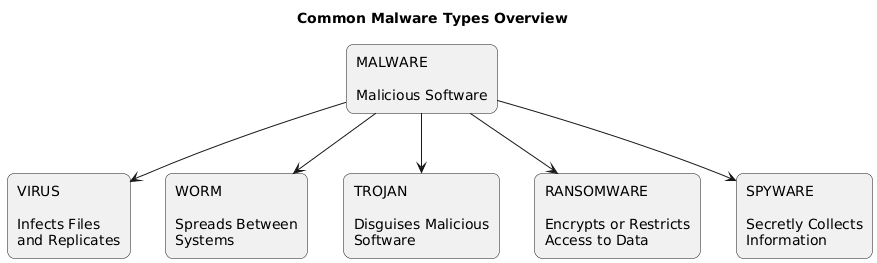
\includegraphics[width=.95\textwidth]{images/malware_types_overview.png}
\caption{Common Malware Types Overview}
\end{figure}

% ============================================================
% MALWARE COMPARISON
% ============================================================

\subsection{Malware Comparison}

\begin{table}[H]
\centering
\small
\renewcommand{\arraystretch}{1.25}

\begin{tabularx}{\textwidth}{
|p{2.2cm}|X|X|X|
}
\hline
\textbf{Malware}
&
\textbf{Main Behavior}
&
\textbf{Typical Impact}
&
\textbf{Basic Protection}
\\
\hline

Virus
&
Infects files and replicates when activated
&
File/system modification
&
Updates and security software
\\
\hline

Worm
&
Replicates and spreads between systems
&
Rapid network/system infection
&
Patching, firewalls, segmentation
\\
\hline

Trojan
&
Disguises malicious software as legitimate software
&
Unauthorized activity
&
Trusted software sources
\\
\hline

Ransomware
&
Encrypts or restricts access to data
&
Loss of data availability
&
Backups and patching
\\
\hline

Spyware
&
Secretly collects information
&
Privacy/information loss
&
Trusted apps and endpoint security
\\
\hline

\end{tabularx}

\caption{Comparison of Common Malware Types}

\end{table}

% ============================================================
% MALWARE MINI PRACTICAL
% ============================================================

\subsection{Mini Practical / Try It Yourself}

A safe malware-awareness activity can be performed without downloading or executing real malware.

\begin{enumerate}
    \item Open the security settings of your operating system.
    \item Check whether real-time protection is enabled.
    \item Check the latest security update.
    \item Review installed applications.
    \item Verify unfamiliar applications before taking action.
\end{enumerate}

\textbf{Safety Note:} Do not download, execute, or interact with real malware for this assignment.

% ============================================================
% MALWARE CYBERSECURITY CONNECTION
% ============================================================

\subsection{Cybersecurity Connection}

Malware knowledge is important for cybersecurity analysts because malware can affect endpoints, networks, applications, and data. Analysts may use endpoint detection tools, security alerts, logs, network traffic, and file activity to investigate suspicious behavior.

% ============================================================
% MALWARE SECURITY RISKS
% ============================================================

\subsection{Security Risks and Protection}

\textbf{Risks:} Unauthorized access, information theft, file destruction, loss of data availability, and spread across connected systems.

\textbf{Protection:} Keep systems updated; use reputable security software; maintain protected backups; use strong authentication; use trusted software sources; avoid suspicious attachments and links; monitor unusual activity.

% ============================================================
% MALWARE QUICK CHECK
% ============================================================

\subsection{Quick Check}

\begin{enumerate}
    \item Which malware attaches to files?
    \item Which malware spreads automatically?
    \item Which disguises itself as legitimate software?
    \item Which commonly encrypts data?
    \item Which secretly collects information?
\end{enumerate}

\textbf{Answers:}

1. Virus.

2. Worm.

3. Trojan.

4. Ransomware.

5. Spyware.

% ============================================================
% TASK 1 SUMMARY
% ============================================================

\subsection{Task 1 Summary}

Viruses infect files, worms spread between systems, Trojans disguise malicious software, ransomware can restrict access to data, and spyware can secretly collect information. Understanding these types helps users recognize threats and helps cybersecurity professionals investigate malicious activity.

% ============================================================
% TASK 2
% ============================================================

\clearpage

\section{Task 2: Understanding Phishing}

\subsection{Introduction}

Phishing is a social-engineering technique in which attackers use deceptive messages, calls, or websites to trick people into revealing sensitive information, clicking harmful links, downloading malicious content, or performing an action that benefits the attacker.

% ============================================================
% WHAT IS PHISHING
% ============================================================

\subsection{What is Phishing?}

\subsubsection{Definition}

Phishing uses deceptive communication to trick a victim into providing sensitive information or performing an unsafe action. Attackers commonly impersonate trusted people, companies, services, or organizations.

\subsubsection{How a Phishing Attack Works}

A typical attack begins when an attacker prepares a deceptive message and delivers it through email, SMS, a phone call, a website, or another communication channel. The victim is encouraged to click, respond, enter credentials, make a payment, or provide sensitive information.

\begin{figure}[H]
\centering
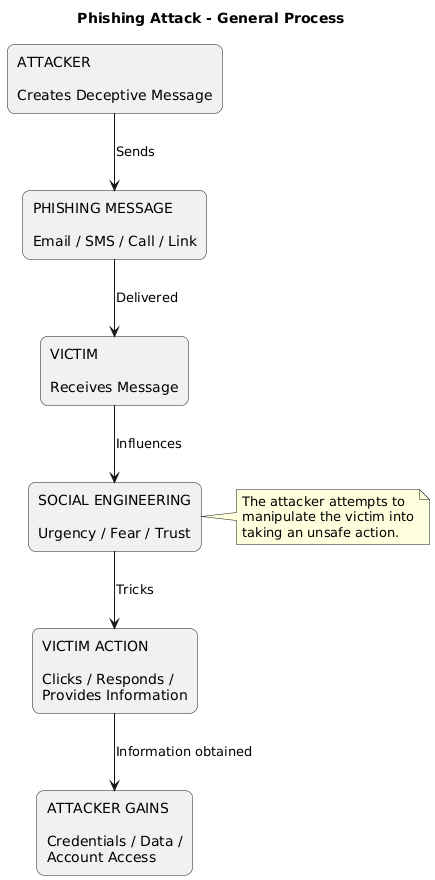
\includegraphics[width=.72\textwidth]{images/phishing_attack_flow.png}
\caption{Phishing Attack -- General Process}
\end{figure}

\subsubsection{Why Do Attackers Use Phishing?}

Attackers use phishing to exploit human decision-making. Successful phishing may steal credentials, obtain personal or financial information, gain account access, deliver malware, redirect users to fraudulent sites, or convince victims to make payments.

\refs
{https://www.nist.gov/itl/smallbusinesscyber/guidance-topic/phishing}
{https://nvlpubs.nist.gov/nistpubs/TechnicalNotes/NIST.TN.2276.pdf}
{https://www.youtube.com/results?search_query=Professor+Messer+phishing}

% ============================================================
% EMAIL PHISHING
% ============================================================

\subsection{Email Phishing}

\subsubsection{Definition}

Email phishing uses deceptive emails to impersonate trusted organizations, companies, or individuals and persuade the recipient to perform an unsafe action.

\subsubsection{How It Works}

The attacker sends an email designed to appear legitimate. It may contain a malicious link, attachment, fake login page, payment request, or request for sensitive information.

\begin{figure}[H]
\centering
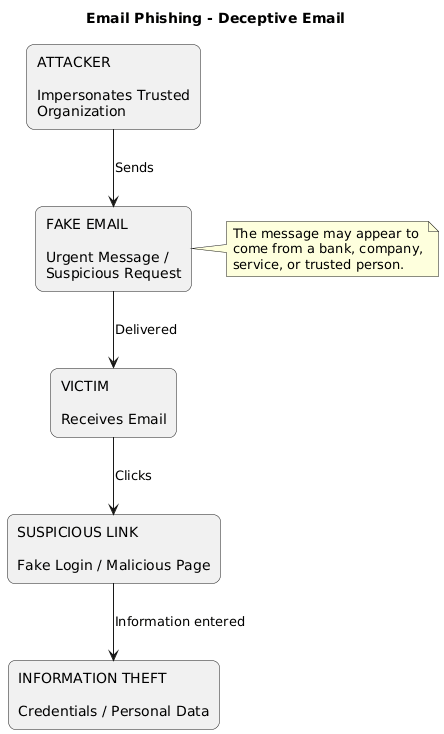
\includegraphics[width=.70\textwidth]{images/email_phishing.png}
\caption{Email Phishing -- Deceptive Email}
\end{figure}

\subsubsection{Real-World Example}

A user may receive an email appearing to come from a bank claiming that immediate account verification is required and providing a fraudulent login link.

\subsubsection{Cybersecurity Connection}

Security teams may use email filtering, URL analysis, threat intelligence, and user reporting to identify suspicious messages.

\subsubsection{Security Risk and Protection}

\textbf{Risk:} A user may disclose credentials or download malicious content.

\textbf{Protection:} Verify the sender; inspect links; avoid unexpected attachments; verify requests through official channels; report suspicious emails.

\refs
{https://consumer.ftc.gov/articles/how-recognize-avoid-phishing-scams}
{https://www.nist.gov/itl/smallbusinesscyber/guidance-topic/phishing}
{https://www.youtube.com/results?search_query=Professor+Messer+phishing}

% ============================================================
% SMISHING
% ============================================================

\subsection{Smishing}

\subsubsection{Definition}

Smishing is phishing conducted through SMS or other text messaging services.

\subsubsection{How It Works}

An attacker sends a text that may appear to come from a bank, delivery company, service provider, or other trusted organization, often containing a link or request for information.

\begin{figure}[H]
\centering
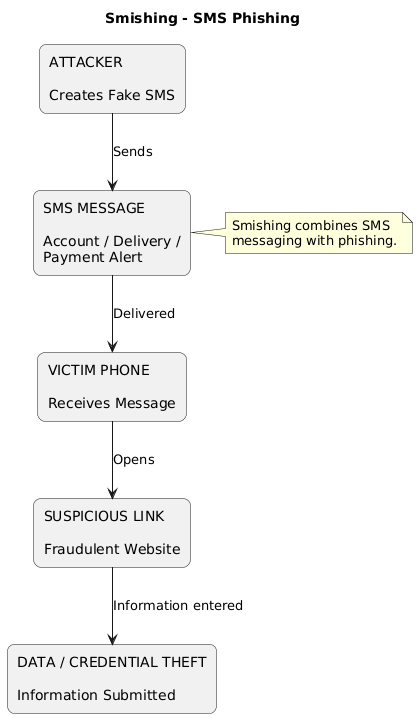
\includegraphics[width=.70\textwidth]{images/smishing.png}
\caption{Smishing -- SMS Phishing}
\end{figure}

\subsubsection{Real-World Example}

A user may receive a text claiming that a package cannot be delivered until a payment or address confirmation is completed.

\subsubsection{Cybersecurity Connection}

Smishing is important to mobile security because users may trust messages received on personal devices.

\subsubsection{Security Risk and Protection}

\textbf{Risk:} A victim may open a malicious link or submit credentials or payment information.

\textbf{Protection:} Do not trust unexpected messages; avoid suspicious links; verify through the official app/site; report suspicious messages; delete after reporting.

\refs
{https://consumer.ftc.gov/articles/how-recognize-avoid-phishing-scams}
{https://www.nist.gov/itl/smallbusinesscyber/guidance-topic/phishing}
{https://www.youtube.com/results?search_query=Professor+Messer+smishing+phishing}

% ============================================================
% VISHING
% ============================================================

\subsection{Vishing}

\subsubsection{Definition}

Vishing, or voice phishing, is phishing conducted through telephone or voice communication.

\subsubsection{How It Works}

The attacker creates a believable urgent situation, such as a supposed security problem or payment issue, and asks the victim for sensitive information.

\begin{figure}[H]
\centering
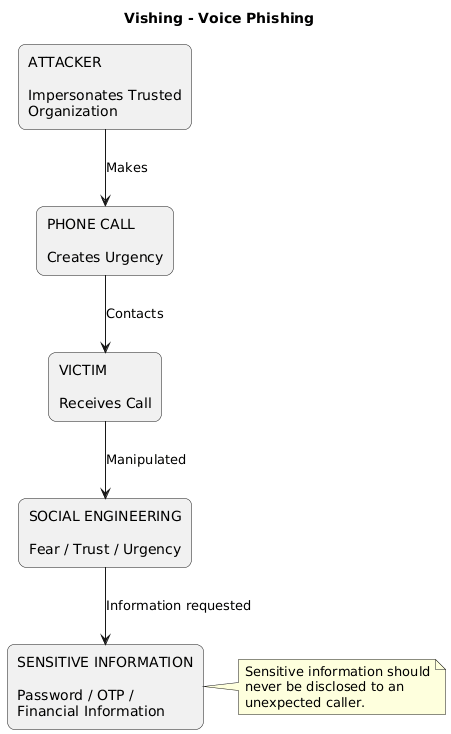
\includegraphics[width=.70\textwidth]{images/vishing.png}
\caption{Vishing -- Voice Phishing}
\end{figure}

\subsubsection{Real-World Example}

A caller may pretend to be from a bank's security department and ask for an OTP, password, or card information.

\subsubsection{Cybersecurity Connection}

Vishing demonstrates how social engineering can operate without malware or technical exploitation. Security awareness helps users recognize impersonation.

\subsubsection{Security Risk and Protection}

\textbf{Risk:} Victims may reveal credentials, financial information, or authentication codes.

\textbf{Protection:} Never disclose passwords or OTPs during unexpected calls; end suspicious calls; use official contact numbers; do not trust caller ID alone; report suspected fraud.

\refs
{https://consumer.ftc.gov/all-scams/phishing-scams}
{https://www.nist.gov/itl/smallbusinesscyber/guidance-topic/phishing}
{https://www.youtube.com/results?search_query=Professor+Messer+social+engineering}

% ============================================================
% FAKE WEBSITE / LINK PHISHING
% ============================================================

\subsection{Fake Website / Link Phishing}

\subsubsection{Definition}

Fake website or link phishing uses deceptive URLs or fraudulent websites that imitate legitimate services to collect credentials or other sensitive data.

\subsubsection{How It Works}

A deceptive link is distributed through email, SMS, social media, or another channel. The victim is directed to a fraudulent website that may visually imitate a legitimate service.

\begin{figure}[H]
\centering
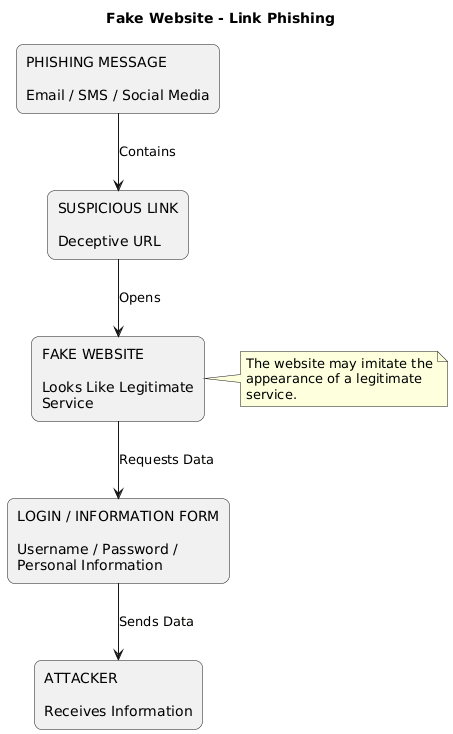
\includegraphics[width=.72\textwidth]{images/fake_website_phishing.png}
\caption{Fake Website -- Link Phishing}
\end{figure}

\subsubsection{Real-World Example}

A phishing message may contain a link that appears to belong to an online service but leads to a fraudulent login page.

\subsubsection{Cybersecurity Connection}

Security teams can analyze URLs, domains, certificates, page content, and reported phishing indicators.

\subsubsection{Security Risk and Protection}

\textbf{Risk:} Entering credentials into a fraudulent website can give attackers access to an account.

\textbf{Protection:} Check the address carefully; avoid unexpected links; use known official websites/apps; enable multi-factor authentication; report fraudulent sites.

\refs
{https://www.nist.gov/itl/smallbusinesscyber/guidance-topic/phishing}
{https://nvlpubs.nist.gov/nistpubs/TechnicalNotes/NIST.TN.2276.pdf}
{https://www.youtube.com/results?search_query=Professor+Messer+phishing}

% ============================================================
% FIVE SIGNS OF PHISHING
% ============================================================

\subsection{Five Common Signs of a Phishing Message}

\begin{enumerate}
    \item \textbf{Suspicious sender:}
    The sender address may not match the claimed organization.

    \item \textbf{Urgent or threatening language:}
    The message pressures the recipient to act immediately.

    \item \textbf{Suspicious link:}
    The URL may not match the expected organization.

    \item \textbf{Request for sensitive information:}
    Passwords, financial information, or authentication codes may be requested.

    \item \textbf{Spelling, grammar, or unusual content:}
    Errors, unusual formatting, or unexpected requests can be warning signs.
\end{enumerate}

\begin{figure}[H]
\centering
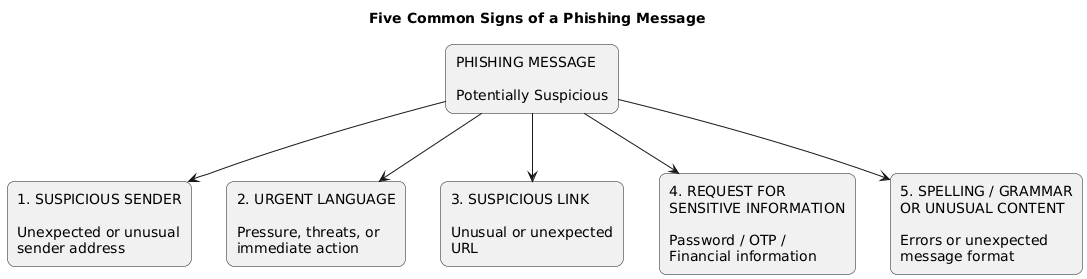
\includegraphics[width=.98\textwidth]{images/phishing_warning_signs.png}
\caption{Five Common Signs of a Phishing Message}
\end{figure}

\refs
{https://www.nist.gov/itl/smallbusinesscyber/guidance-topic/phishing}
{https://nvlpubs.nist.gov/nistpubs/TechnicalNotes/NIST.TN.2276.pdf}
{https://www.youtube.com/results?search_query=NIST+phishing+awareness}

% ============================================================
% PHISHING COMPARISON
% ============================================================



\subsection{Phishing Types Comparison}

\begin{table}[H]
\centering
\small
\renewcommand{\arraystretch}{1.25}

\begin{tabularx}{\textwidth}{
|p{2.4cm}|p{2.2cm}|X|X|
}
\hline

\textbf{Type}
&
\textbf{Channel}
&
\textbf{Common Technique}
&
\textbf{Typical Target}
\\
\hline

Email Phishing
&
Email
&
Fake messages, links, attachments
&
Credentials and sensitive information
\\
\hline

Smishing
&
SMS / Text
&
Fake delivery, account, or payment messages
&
Mobile users and account information
\\
\hline

Vishing
&
Voice / Phone
&
Impersonation and urgent requests
&
Credentials, financial information, OTPs
\\
\hline

Fake Website / Link Phishing
&
Web / Links
&
Fraudulent websites and deceptive URLs
&
Login credentials and personal information
\\
\hline

\end{tabularx}

\caption{Comparison of Common Phishing Types}

\end{table}

% ============================================================
% PHISHING MINI PRACTICAL
% ============================================================

\subsection{Mini Practical / Try It Yourself}

A safe phishing-awareness activity can be performed without interacting with a real phishing website.

\begin{enumerate}
    \item Find a phishing-awareness example from NIST, FTC, or another recognized cybersecurity-awareness organization.
    \item Examine sender information.
    \item Identify suspicious links or requests without opening them.
    \item Identify urgency, threats, or unusual wording.
    \item Identify requests for sensitive information.
    \item Record the warning signs.
\end{enumerate}

\textbf{Safety Note:} Do not click suspicious links, download unknown attachments, submit personal information, or interact with real phishing websites.

% ============================================================
% PHISHING CYBERSECURITY CONNECTION
% ============================================================

\subsection{Cybersecurity Connection}

Phishing is important to cybersecurity because attackers can use social engineering to bypass technical controls by manipulating users. Security teams may use email security gateways, spam filters, URL analysis, threat intelligence, endpoint security tools, and user reporting.

% ============================================================
% PHISHING SECURITY RISKS
% ============================================================

\subsection{Security Risks and Protection}

\textbf{Risks:} Credential theft, financial fraud, account compromise, malware infection, identity theft, and unauthorized access.

\textbf{Protection:} Stop and verify unexpected requests; do not click suspicious links or attachments; use multi-factor authentication; verify through official channels; report suspicious messages; keep devices updated.

\refs
{https://consumer.ftc.gov/articles/how-recognize-avoid-phishing-scams}
{https://www.nist.gov/itl/smallbusinesscyber/guidance-topic/phishing}
{https://www.youtube.com/results?search_query=NIST+phishing+awareness}

% ============================================================
% SAFE RESPONSE
% ============================================================

\subsection{Safe Response to a Suspicious Message}

\begin{figure}[H]
\centering
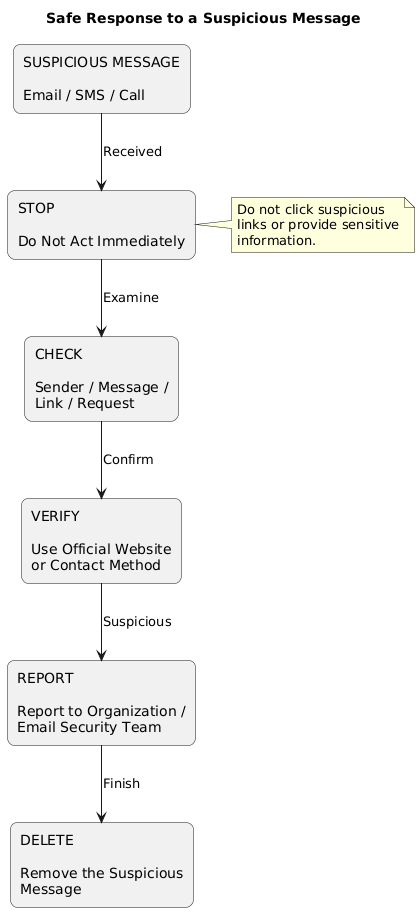
\includegraphics[width=.62\textwidth]{images/phishing_protection.png}
\caption{Safe Response to a Suspicious Message}
\end{figure}

% ============================================================
% QUICK CHECK
% ============================================================

\subsection{Quick Check}

\begin{enumerate}
    \item What is phishing?
    \item Why do attackers use phishing?
    \item What is the difference between phishing and smishing?
    \item What does vishing use?
    \item Name five warning signs of phishing.
\end{enumerate}

\textbf{Answers:}

1. A social-engineering attack using deceptive communication.

2. To obtain information, access, money, or deliver malicious content.

3. Smishing specifically uses SMS/text messages.

4. Voice or telephone communication.

5. Suspicious sender, urgent language, suspicious link, request for sensitive information, and unusual spelling/grammar/content.

% ============================================================
% TASK 2 SUMMARY
% ============================================================

\subsection{Task 2 Summary}

Phishing is a social-engineering technique that manipulates users into clicking harmful links, opening malicious content, or revealing sensitive information. Email phishing, smishing, vishing, and fake website/link phishing use different channels but share the objective of deceiving the victim. Recognizing common warning signs helps users avoid unsafe actions.

% ============================================================
% END
% ============================================================


% ============================================================
% TASK 3
% ============================================================

\section{Task 3: Identify a Phishing Message}

\subsection{Introduction}

Phishing messages are designed to appear trustworthy while attempting
to persuade a recipient to click a link, open an attachment, provide
sensitive information, or perform another action. A safe analysis
should therefore focus on observable warning signs rather than on
interacting with the suspicious message.

For this task, two publicly documented phishing examples from
security-awareness resources were reviewed. The examples are used only
for educational analysis. Suspicious links, attachments, phone numbers,
and websites should not be opened or contacted during the analysis.

\subsection{Phishing Message Analysis Process}

A phishing message can be examined systematically by checking the
sender, links, language, requested information, and other unusual
content. After identifying the warning signs, the safest response is
to verify independently, report the message when appropriate, and
delete it.

\begin{figure}[H]
\centering
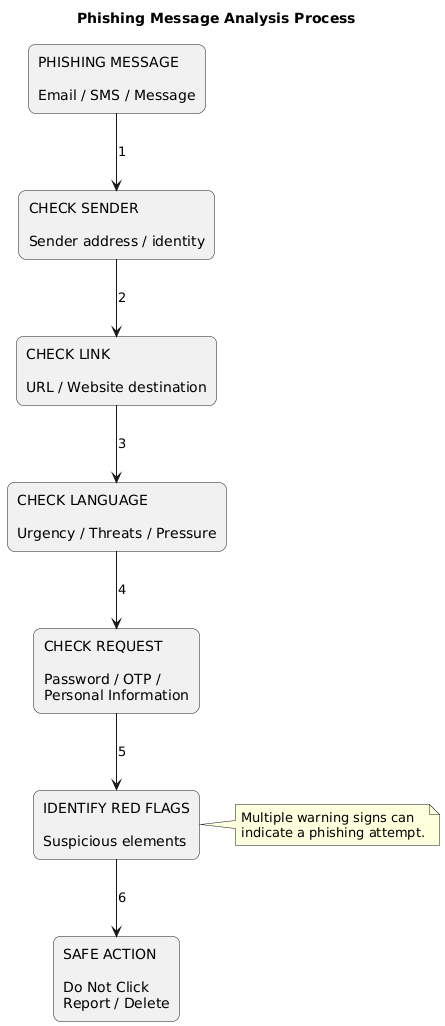
\includegraphics[width=0.48\textwidth]{images/phishing_analysis_flow.png}
\caption{Phishing Message Analysis Process}
\label{fig:phishing-analysis}
\end{figure}
\FloatBarrier

\subsection{Phishing Identification Checklist}

The following checklist groups common indicators that can be reviewed
without interacting with a suspicious message.

\begin{figure}[H]
\centering
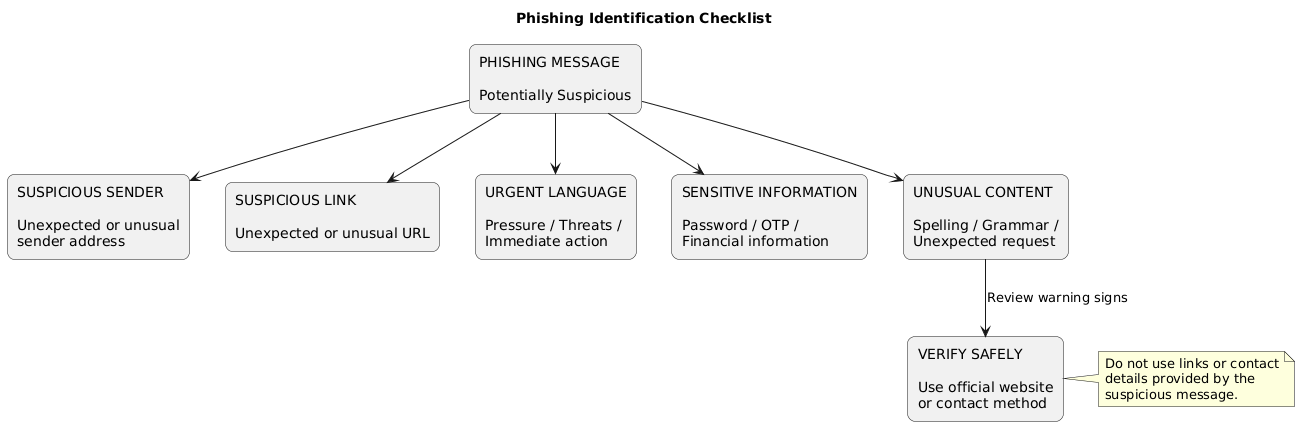
\includegraphics[width=0.98\textwidth]{images/phishing_identification_checklist.png}
\caption{Phishing Identification Checklist}
\label{fig:phishing-checklist}
\end{figure}
\FloatBarrier

\subsection{Public Example 1: Fake MetaMask Phishing Email}

The U.S. Federal Trade Commission (FTC) published examples of fake
MetaMask and PayPal messages. The MetaMask message falsely claimed that
the recipient's cryptocurrency wallet was blocked and created pressure
to act quickly by clicking a link and updating the wallet. The FTC
warned that unexpected messages asking users to act quickly, click a
link, or call a number are common phishing patterns.

\begin{table}[H]
\centering
\small
\renewcommand{\arraystretch}{1.35}
\begin{tabular}{|p{4.0cm}|p{9.2cm}|}
\hline
\textbf{Indicator} & \textbf{Analysis}\\
\hline
Suspicious sender & The message impersonates a trusted service. The sender identity should not be accepted only because the message uses a familiar company name.\\
\hline
Suspicious link & The message asks the recipient to click a link to update or resolve the wallet problem. The link should not be opened.\\
\hline
Urgent / threatening language & It claims the wallet is blocked and suggests that the recipient must act quickly or risk losing cryptocurrency.\\
\hline
Spelling / grammar & Poor writing is not required for a message to be phishing. Modern phishing messages may be professionally written, so grammar alone is not a reliable test.\\
\hline
Request for personal information & The requested wallet update is intended to make the recipient interact with a fraudulent destination and potentially expose sensitive information.\\
\hline
Other suspicious element & The problem is unexpected and creates pressure to solve it through the message itself instead of independently verifying the account.\\
\hline
\end{tabular}
\caption{Analysis of the FTC MetaMask phishing example}
\label{tab:metamask-analysis}
\end{table}

\textbf{Why it should not be trusted:} The message combines impersonation,
urgency, and a request to click a link. A safer approach is to open the
official service independently or use a known contact method instead of
using information supplied by the message.

\referenceblock{FTC, ``Those urgent emails from MetaMask and PayPal are phishing scams.''}{https://consumer.ftc.gov/comment/181991}

\subsection{Public Example 2: Fake Direct-Deposit Phishing Email}

NIST's phishing-awareness material includes a sample direct-deposit
phishing email. The example appears to come from an individual and
claims that the sender has changed banks and needs direct-deposit
information updated before the previous account is closed. It creates
pressure to provide assistance promptly.

\begin{table}[H]
\centering
\small
\renewcommand{\arraystretch}{1.35}
\begin{tabular}{|p{4.0cm}|p{9.2cm}|}
\hline
\textbf{Indicator} & \textbf{Analysis}\\
\hline
Suspicious sender & The educational example shows an email from an address that does not provide sufficient assurance that the sender is really the person represented. Sender identity should be independently verified.\\
\hline
Suspicious link & The published description does not identify a specific embedded URL as the main indicator. The absence of a visible link does not make the request trustworthy.\\
\hline
Urgent / threatening language & The sender says the previous bank account will be closed in a few days and asks for prompt assistance, creating time pressure.\\
\hline
Spelling / grammar & The example is relatively well written. This demonstrates that correct spelling and grammar do not prove that an email is legitimate.\\
\hline
Request for personal information & The message attempts to obtain information related to direct-deposit banking details, which is highly sensitive.\\
\hline
Other suspicious element & A request to change payment or banking information should be independently verified through a trusted organizational process.\\
\hline
\end{tabular}
\caption{Analysis of the NIST direct-deposit phishing example}
\label{tab:direct-deposit-analysis}
\end{table}

\textbf{Why it should not be trusted:} A request involving salary or
banking information is high impact. The recipient should verify the
request using a known phone number, internal system, or previously
established contact method rather than replying to the suspicious
message.

\referenceblock{NIST, ``Phishing Cues-SOUPS Poster'' -- sample direct-deposit phishing email.}{https://tsapps.nist.gov/publication/get_pdf.cfm?pub_id=956178}

\subsection{Comparison of the Two Phishing Examples}

\begin{table}[H]
\centering
\small
\renewcommand{\arraystretch}{1.35}
\begin{tabular}{|p{3.0cm}|p{5.0cm}|p{5.0cm}|}
\hline
\textbf{Indicator} & \textbf{Example 1: MetaMask} & \textbf{Example 2: Direct Deposit}\\
\hline
Impersonation & Trusted cryptocurrency service & Individual / organizational identity\\
\hline
Pressure & Act quickly to avoid loss of cryptocurrency & Act promptly before an account is closed\\
\hline
Sensitive target & Wallet/account information & Banking and payroll information\\
\hline
Link involvement & Link requested to resolve the fake problem & No specific embedded link identified in the published description\\
\hline
Safe response & Independently verify the wallet/service & Independently verify through a trusted organizational channel\\
\hline
\end{tabular}
\caption{Comparison of two publicly documented phishing examples}
\label{tab:phishing-comparison}
\end{table}

\subsection{Cybersecurity Connection}

Phishing is directly connected to identity theft, credential theft,
malware delivery, financial fraud, and unauthorized account access.
A successful phishing attempt can also become the first stage of a
larger attack. Security awareness therefore acts as an important
preventive control alongside technical controls such as spam filters,
endpoint security, multi-factor authentication, and email protection.

\subsection{Security Risks and Basic Protection}

\textbf{Major Risks:}
\begin{itemize}
    \item Theft of usernames, passwords, OTPs, and financial information.
    \item Installation of malware through malicious links or attachments.
    \item Account takeover after stolen credentials are reused.
    \item Financial loss and identity theft.
    \item Further compromise of an organization after an employee is deceived.
\end{itemize}

\textbf{Basic Protection:}
\begin{itemize}
    \item Do not click unexpected links or open unexpected attachments.
    \item Verify suspicious requests using an independently known contact method.
    \item Use multi-factor authentication on important accounts.
    \item Report suspicious messages through the appropriate reporting mechanism.
    \item Delete phishing messages after reporting and documenting them when required.
\end{itemize}

\referenceblock{CISA, ``Avoid Phishing Scams with Three Simple Tips.''}{https://www.cisa.gov/sites/default/files/2024-09/Secure-Our-World-Phishing-Tip-Sheet.pdf}

\paperblock{NIST, ``Phishing'' -- Small Business Cybersecurity Guidance}{https://www.nist.gov/itl/smallbusinesscyber/guidance-topic/phishing}

\videoblock{1}{Professor Messer -- Phishing and Social Engineering}{https://www.youtube.com/results?search_query=Professor+Messer+phishing+social+engineering}

\subsection{Quick Check}

\begin{enumerate}
    \item Why should a suspicious link not be opened during analysis?
    \item Name two common warning signs of a phishing message.
    \item Why should a request for banking or password information be verified independently?
    \item Is poor grammar required for a message to be phishing?
\end{enumerate}

\subsubsection*{Answers}

\begin{enumerate}
    \item Because the link may lead to a fraudulent website or malicious content.
    \item Examples include an unusual sender, suspicious link, urgent language, unexpected attachment, or request for sensitive information.
    \item Because the message may be impersonating a trusted person or organization and could be attempting to steal sensitive information.
    \item No. A phishing message can be professionally written, so grammar alone is not a reliable indicator.
\end{enumerate}

\subsection{Task 3 Summary}

The two public examples demonstrate that phishing messages often rely
on impersonation, urgency, unexpected requests, suspicious links, and
attempts to obtain sensitive information. A safe analysis does not
require interacting with the suspicious content. Instead, the message
should be examined for warning signs and verified through an
independent trusted channel.

% ============================================================
% TASK 4
% ============================================================

\section{Task 4: Malware Prevention}

\subsection{Introduction}

Malware prevention combines technical controls, safe software habits,
secure account practices, backups, and user awareness. No single
control eliminates every malware risk, so several protective measures
should be used together.

\subsection{Malware Prevention -- Overall Security Process}

A basic prevention process begins with keeping the device updated and
using security software. Trusted applications, safe downloads,
careful handling of attachments, strong authentication, and backups
further reduce the likelihood or impact of malware incidents.

\begin{figure}[H]
\centering
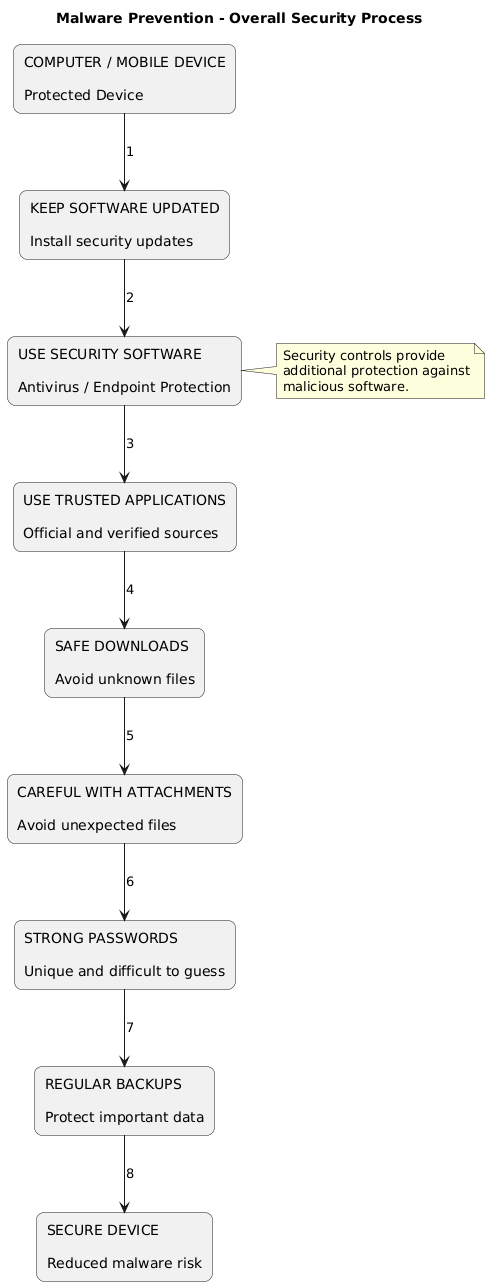
\includegraphics[width=0.36\textwidth]{images/malware_prevention_overall.png}
\caption{Malware Prevention -- Overall Security Process}
\label{fig:malware-overall}
\end{figure}
\FloatBarrier

\subsection{Ten Malware Prevention Practices}

The following ten practices provide a practical baseline for reducing
malware risk on computers and mobile devices.

\begin{figure}[H]
\centering
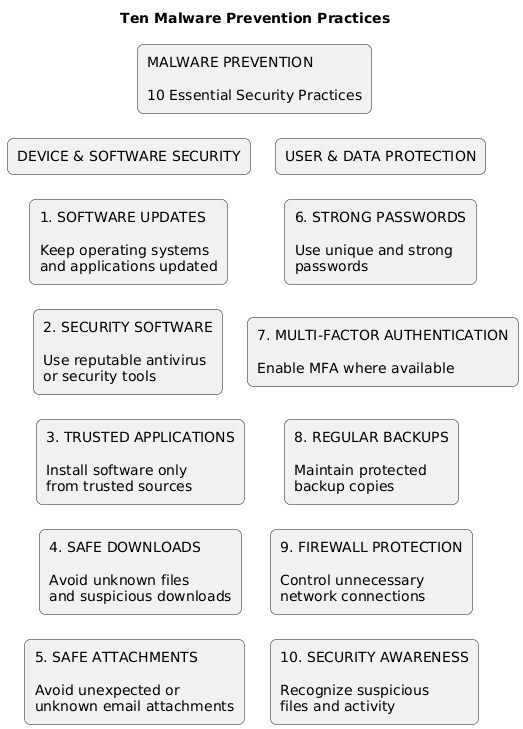
\includegraphics[width=0.70\textwidth]{images/ten_malware_prevention_practices.png}
\caption{Ten Malware Prevention Practices}
\label{fig:ten-malware-practices}
\end{figure}
\FloatBarrier

\begin{enumerate}
    \item \textbf{Keep software updated} -- Install operating-system and application security updates.
    \item \textbf{Use security software} -- Use reputable antivirus or endpoint protection where appropriate.
    \item \textbf{Use trusted applications} -- Install software from official or otherwise trusted sources.
    \item \textbf{Use safe downloads} -- Avoid unknown files and suspicious download websites.
    \item \textbf{Be careful with attachments} -- Do not open unexpected or suspicious files.
    \item \textbf{Use strong passwords} -- Use unique passwords or passphrases for important accounts.
    \item \textbf{Enable multi-factor authentication} -- Add an additional verification factor where supported.
    \item \textbf{Maintain regular backups} -- Keep protected copies of important data.
    \item \textbf{Use firewall protection} -- Control unnecessary network connections and exposure.
    \item \textbf{Maintain security awareness} -- Recognize suspicious files, links, prompts, and behavior.
\end{enumerate}

\subsection{Detailed Explanation of Five Practices}

\subsubsection{1. Keep Software Updated}

Software updates frequently contain security fixes that address known
vulnerabilities. Keeping the operating system, browser, applications,
and security tools updated reduces exposure to vulnerabilities that
attackers may attempt to exploit.

\textbf{Practical action:} Enable automatic updates where appropriate
and regularly check for updates for software that does not update
automatically.

\subsubsection{2. Use Security Software}

Reputable antivirus or endpoint-security software can help detect,
block, quarantine, or remove malicious software. Security software is
not a replacement for safe behavior, but it provides an additional
layer of protection.

\textbf{Practical action:} Keep security software active and updated,
and perform scans when suspicious behavior is observed.

\subsubsection{3. Use Trusted Applications and Safe Downloads}

Applications should be obtained from official stores, known vendors,
or other trusted sources. Unofficial or modified installers can contain
malware or unwanted software. Users should also verify the publisher
and download source before installation.

\textbf{Practical action:} Check the official website or trusted app
store, verify the publisher, and avoid suspicious download portals.

\subsubsection{4. Avoid Unknown Attachments}

Malware can be delivered through malicious email attachments and other
unexpected files. A file that appears to be an invoice, document, or
image may contain malicious content or direct the user to a harmful
website.

\textbf{Practical action:} Verify unexpected attachments through a
separate trusted channel before opening them.

\subsubsection{5. Maintain Regular Backups}

Backups reduce the impact of data loss caused by malware, accidental
deletion, hardware failure, or ransomware. A useful backup strategy
keeps copies protected from unauthorized modification or deletion.

\textbf{Practical action:} Back up important files regularly and
periodically verify that the backup can actually be restored.

\subsection{Malware Backup and Recovery Process}

Backups are particularly important when malware causes data loss or
makes files unavailable. A safe recovery process isolates the affected
device, removes or rebuilds the compromised system, and restores data
from a trusted backup.

\begin{figure}[H]
\centering
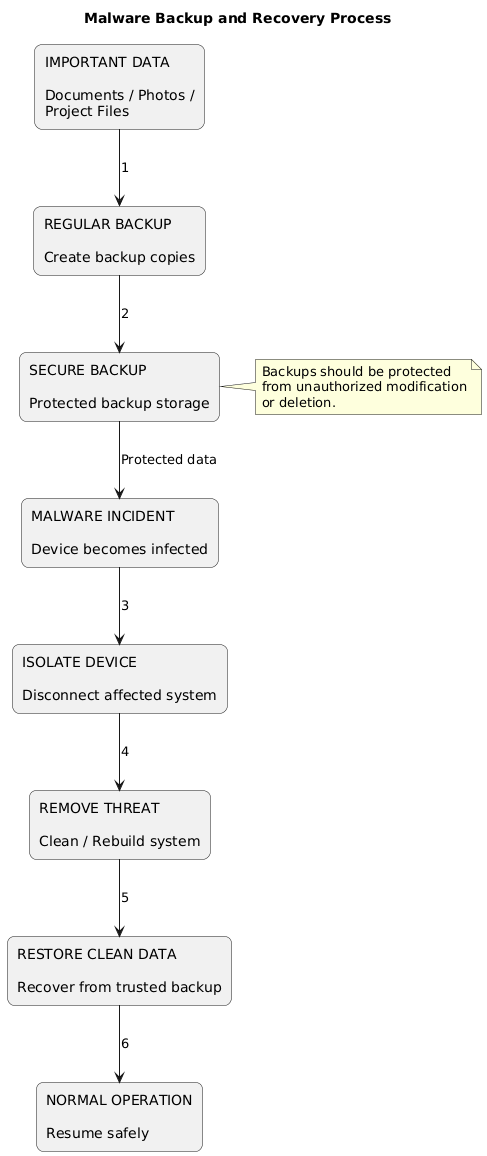
\includegraphics[width=0.32\textwidth]{images/malware_backup_recovery.png}
\caption{Malware Backup and Recovery Process}
\label{fig:backup-recovery}
\end{figure}
\FloatBarrier

\textbf{Important point:} A backup that remains permanently connected
and writable by the infected system may also be affected by malware.
Backups should therefore be protected against unauthorized modification
or deletion.

\subsection{Safe Software Download and Installation}

Software should be obtained from a trusted source and checked before
installation. If the source is suspicious or cannot be verified, the
safest action is to stop rather than continue with the installation.

\begin{figure}[H]
\centering
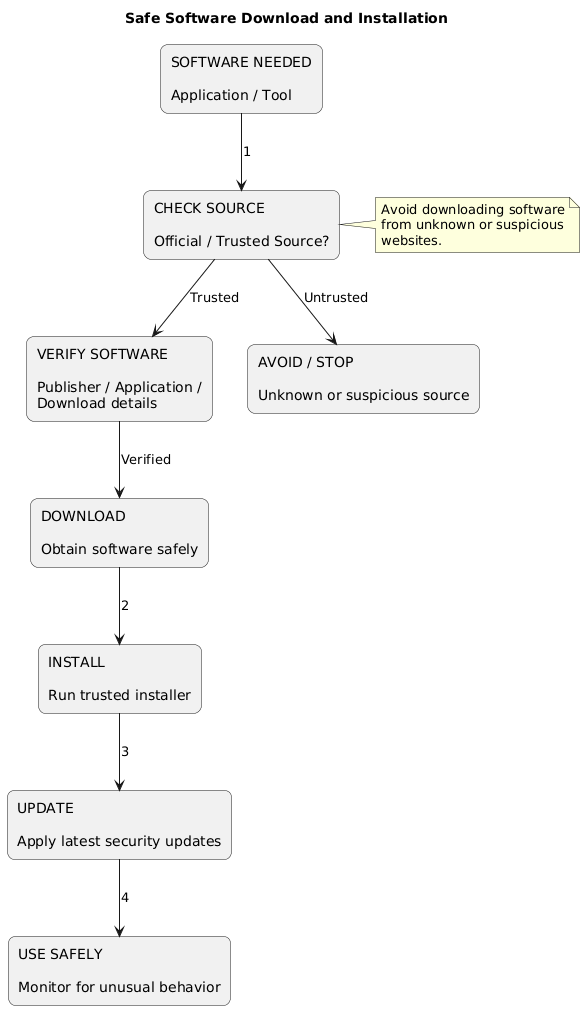
\includegraphics[width=0.48\textwidth]{images/safe_software_download.png}
\caption{Safe Software Download and Installation}
\label{fig:safe-download}
\end{figure}
\FloatBarrier

\referenceblock{CISA, ``Secure Our World -- Malware and software security guidance.''}{https://www.cisa.gov/secure-our-world}

\paperblock{NIST, ``Cybersecurity Framework (CSF) 2.0'' -- protection, detection, response, and recovery concepts}{https://www.nist.gov/cyberframework}

\videoblock{2}{Professor Messer -- Malware and Malware Prevention}{https://www.youtube.com/results?search_query=Professor+Messer+malware+prevention}

\subsection{Cybersecurity Connection}

Malware prevention is a layered security activity. Updates reduce
known vulnerabilities, security software provides detection, trusted
software sources reduce supply-chain and malicious-download risks,
backups support recovery, firewalls reduce unnecessary exposure, and
security awareness reduces unsafe user actions.

These controls correspond to the broader cybersecurity cycle of
protecting systems, detecting suspicious activity, responding to
incidents, and recovering from security events.

\subsection{Security Risks and Basic Protection}

\begin{table}[H]
\centering
\small
\renewcommand{\arraystretch}{1.35}
\begin{tabular}{|p{4.0cm}|p{4.5cm}|p{4.5cm}|}
\hline
\textbf{Risk} & \textbf{Possible Impact} & \textbf{Basic Protection}\\
\hline
Unpatched software & Exploitation of known vulnerabilities & Apply security updates\\
\hline
Malicious download & Malware infection & Use trusted sources and verify software\\
\hline
Malicious attachment & Malware execution or credential theft & Verify unexpected attachments before opening\\
\hline
Weak authentication & Account compromise & Use strong unique passwords and MFA\\
\hline
Data loss / ransomware & Loss or encryption of important files & Maintain protected backups\\
\hline
Unnecessary network exposure & Increased attack surface & Use firewall controls and secure configurations\\
\hline
User error & Unsafe execution or disclosure & Maintain security awareness and training\\
\hline
\end{tabular}
\caption{Common malware risks and basic protection}
\label{tab:malware-risks}
\end{table}

\subsection{Mini Practical: Safe Software Verification}

A simple practical activity can be performed without downloading
unknown software.

\begin{enumerate}
    \item Select a commonly used application that is already installed or that you legitimately need.
    \item Locate the official vendor website or trusted application store.
    \item Check the publisher or developer name.
    \item Compare the software name and version information with the official source.
    \item Do not install the application if the source, publisher, or download details appear suspicious.
\end{enumerate}

\textbf{Security Note:} The practical should not involve executing an
unknown file or visiting a suspicious download site. The objective is
to practice safe verification, not to test malware.

\referenceblock{CISA, ``Avoiding Social Engineering and Phishing'' -- safe handling of suspicious content.}{https://www.cisa.gov/topics/cyber-threats-and-advisories/social-engineering}

\subsection{Quick Check}

\begin{enumerate}
    \item Why are software updates important for malware prevention?
    \item Why should software be downloaded from trusted sources?
    \item How can backups reduce the impact of ransomware or data loss?
    \item Why are strong passwords and MFA useful against malware-related account compromise?
    \item Why should unexpected attachments be verified before opening?
\end{enumerate}

\subsubsection*{Answers}

\begin{enumerate}
    \item Updates can fix known security vulnerabilities that attackers may exploit.
    \item Trusted sources reduce the chance of installing modified, malicious, or unwanted software.
    \item Backups provide clean copies of important data that can be restored after an incident.
    \item They make unauthorized account access more difficult, even if a password is exposed.
    \item An unexpected attachment may contain malicious content or lead to further compromise.
\end{enumerate}

\subsection{Task 4 Summary}

Malware prevention requires multiple layers of protection rather than
one security tool. Keeping software updated, using security software,
choosing trusted applications and downloads, handling attachments
carefully, protecting accounts, maintaining backups, using firewalls,
and developing security awareness all contribute to reducing malware
risk.

% ============================================================
% DOCUMENTATION REFERENCES
% ============================================================

\Needspace{5cm}
\subsection{Documentation References}

\begin{enumerate}
    \item CISA -- Secure Our World and phishing-awareness guidance.
    \item FTC Consumer Advice -- phishing and scam-awareness guidance.
    \item NIST -- Phishing guidance and phishing-awareness examples.
    \item NIST Cybersecurity Framework 2.0.
\end{enumerate}

\Needspace{4cm}
\subsection{YouTube Learning References}

\begin{enumerate}
    \item Professor Messer -- Phishing and Social Engineering.
    \item Professor Messer -- Malware and Malware Prevention.
\end{enumerate}


% ============================================================
% TASK 5
% ============================================================

\section{Task 5: Security Awareness Scenario}

\subsection{Introduction}

Security awareness helps users recognize suspicious messages before they become security incidents. Phishing attacks often rely on urgency, fear, impersonation, and requests for sensitive information. This scenario demonstrates how a user should respond when receiving a suspicious account-security message.

\subsection{Security Awareness Scenario}

Consider the following fictional message:

\begin{quote}
\textbf{Account Security Alert}\par
Your account will be permanently blocked within \textbf{24 hours} unless you verify your password. Please use the verification link provided in the message to confirm your account.
\end{quote}

The message creates urgency and directs the recipient to take an authentication-related action through the provided link. The scenario represents a common social-engineering situation in which an attacker attempts to create fear of account loss and pressure the recipient into revealing credentials or visiting a fraudulent website.

\subsection{Security Awareness Scenario Response Process}

A safe response should stop the interaction first, identify the warning signs, verify the situation independently, and report the suspicious message through the appropriate channel.

\begin{figure}[H]
\centering
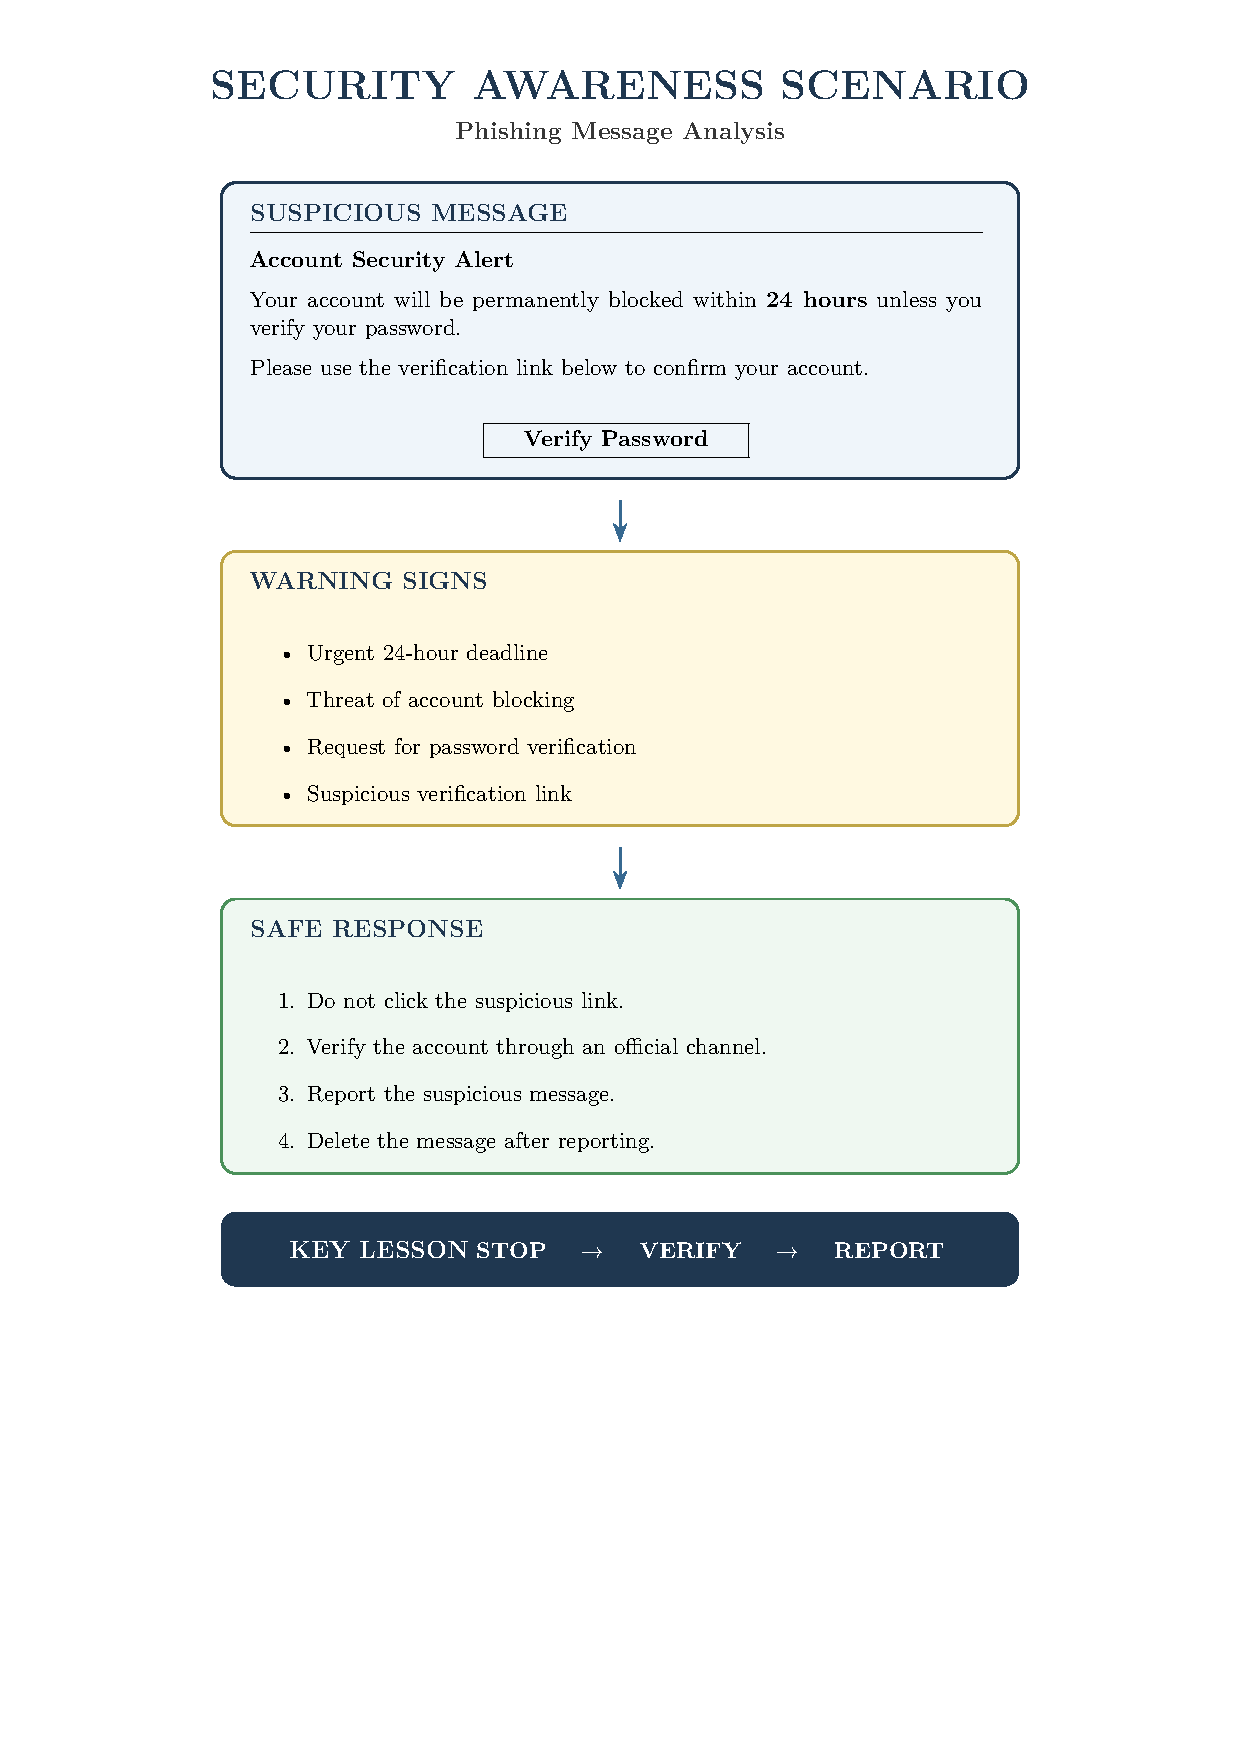
\includegraphics[width=0.82\textwidth]{images/security_awareness_scenario.pdf}
\caption{Security Awareness Scenario Response Process}
\end{figure}

\subsection{What Type of Attack Is This?}

The scenario is a \textbf{phishing attack using social engineering}. The attacker attempts to create urgency and fear of account loss so that the recipient will follow a malicious link and potentially disclose a password or other authentication information.

\subsection{Warning Signs}

\begin{enumerate}
    \item \textbf{Urgent deadline:} The recipient is told that the account will be blocked within 24 hours.
    \item \textbf{Threat of account loss:} The message uses a negative consequence to pressure the recipient.
    \item \textbf{Password request:} A legitimate service should not require a user to disclose a password through an unexpected email link.
    \item \textbf{Suspicious link:} The recipient is instructed to use a link supplied by the message rather than independently accessing the service.
    \item \textbf{Unexpected authentication request:} The request concerns sensitive account information and should be verified before any action is taken.
\end{enumerate}

\subsection{What Should the Recipient Do?}

\begin{itemize}
    \item Do not click the link in the suspicious email.
    \item Do not enter a password, OTP, recovery code, or other sensitive information.
    \item Open the official application or manually enter the known official website address.
    \item Check the account status through the trusted service rather than through the email.
    \item If necessary, contact the organization using a previously known or independently verified contact method.
    \item Report the message through the organization's phishing-reporting mechanism.
    \item Delete the message after reporting and preserve relevant evidence if instructed by the organization.
\end{itemize}

\subsection{What Should the Recipient NOT Do?}

\begin{itemize}
    \item Do not click the suspicious link just to see where it goes.
    \item Do not reply to the sender to verify the request.
    \item Do not provide passwords, OTPs, payment information, or recovery codes.
    \item Do not download or open unexpected attachments.
    \item Do not allow the deadline or threatening language to force an immediate decision.
\end{itemize}

\subsection{Reporting Method}

The suspicious email should be reported using the organization's established phishing-reporting procedure. Depending on the environment, this may be an email-security reporting button, a security operations mailbox, a help-desk process, or another approved reporting channel. The recipient should follow the organization's documented procedure rather than replying to the suspicious sender.

\subsection{Cybersecurity Connection}

This scenario demonstrates how security awareness supports technical security controls. A user who recognizes urgency, impersonation, suspicious links, and credential requests can prevent an initial phishing attempt from becoming credential theft or account compromise. In a security operations environment, reported messages can also provide indicators for investigation, filtering, and incident response.

\subsection{Security Risks and Protection}

\begin{table}[H]
\centering\small
\begin{tabularx}{\textwidth}{|p{3.1cm}|X|X|}
\hline
\textbf{Warning Sign} & \textbf{Possible Risk} & \textbf{Protection}\\\hline
24-hour deadline & Recipient acts without verification & Stop and verify independently\\\hline
Account-blocking threat & Fear-based social engineering & Do not allow pressure to override verification\\\hline
Password request & Credential theft & Never provide passwords through unexpected messages\\\hline
Suspicious link & Fraudulent login page or malicious content & Access the official service independently\\\hline
Unexpected email & Impersonation or unauthorized request & Confirm through a known contact method\\\hline
\end{tabularx}
\caption{Warning Signs and Protective Responses in the Scenario}
\end{table}

\subsection{Mini Practical / Try It Yourself}

Use a fictional phishing message and safely identify its warning signs without opening any suspicious links or attachments.

\begin{enumerate}
    \item Identify the sender and determine whether the message was expected.
    \item Look for urgent deadlines or threatening language.
    \item Identify any request for passwords, OTPs, recovery codes, or payment information.
    \item Inspect the visible destination of a link without opening it.
    \item Record the warning signs and describe the safest response.
\end{enumerate}

\textbf{Safety Note:} Do not click suspicious links, download unknown attachments, submit credentials, or interact with real phishing websites.

\subsection{Documentation References}

\begin{enumerate}
    \item CISA -- phishing-awareness and social-engineering guidance: \url{https://www.cisa.gov/topics/cyber-threats-and-advisories/social-engineering}
    \item NIST -- Phishing, Small Business Cybersecurity Guidance: \url{https://www.nist.gov/itl/smallbusinesscyber/guidance-topic/phishing}
\end{enumerate}

\subsection{YouTube Learning Reference}

\textbf{S.No. 5:} Professor Messer -- Social Engineering and Phishing Awareness.\\
\url{https://www.youtube.com/results?search_query=Professor+Messer+social+engineering+phishing}

\subsection{Quick Check}

\begin{enumerate}
    \item What makes the 24-hour deadline suspicious?
    \item Why should the password-verification link not be used?
    \item What is a safe way to check whether the account is actually at risk?
    \item Where should the suspicious message be reported?
\end{enumerate}

\textbf{Answers}
\begin{enumerate}
    \item It creates urgency and pressure to act before the recipient can verify the request.
    \item It may lead to a fraudulent website or other malicious content designed to steal credentials.
    \item Access the official service independently through a known website, application, or trusted contact method.
    \item It should be reported through the organization's approved phishing-reporting or security-support channel.
\end{enumerate}

\subsection{Task 5 Summary}

The scenario shows how a phishing message can use urgency, threats, and credential requests to influence a recipient. The safest response is to stop, avoid interacting with the suspicious content, verify independently, report the message, and follow the organization's security procedure.

\clearpage

% ============================================================
% TASK 6
% ============================================================

\section{Task 6: Security Awareness Activity}

\subsection{Cyber Security Awareness Poster}

The following poster presents practical security-awareness messages that can be applied to everyday computer and mobile-device use. The poster focuses on preventing common mistakes that can lead to account compromise, malware infection, or data exposure.

\begin{figure}[H]
\centering
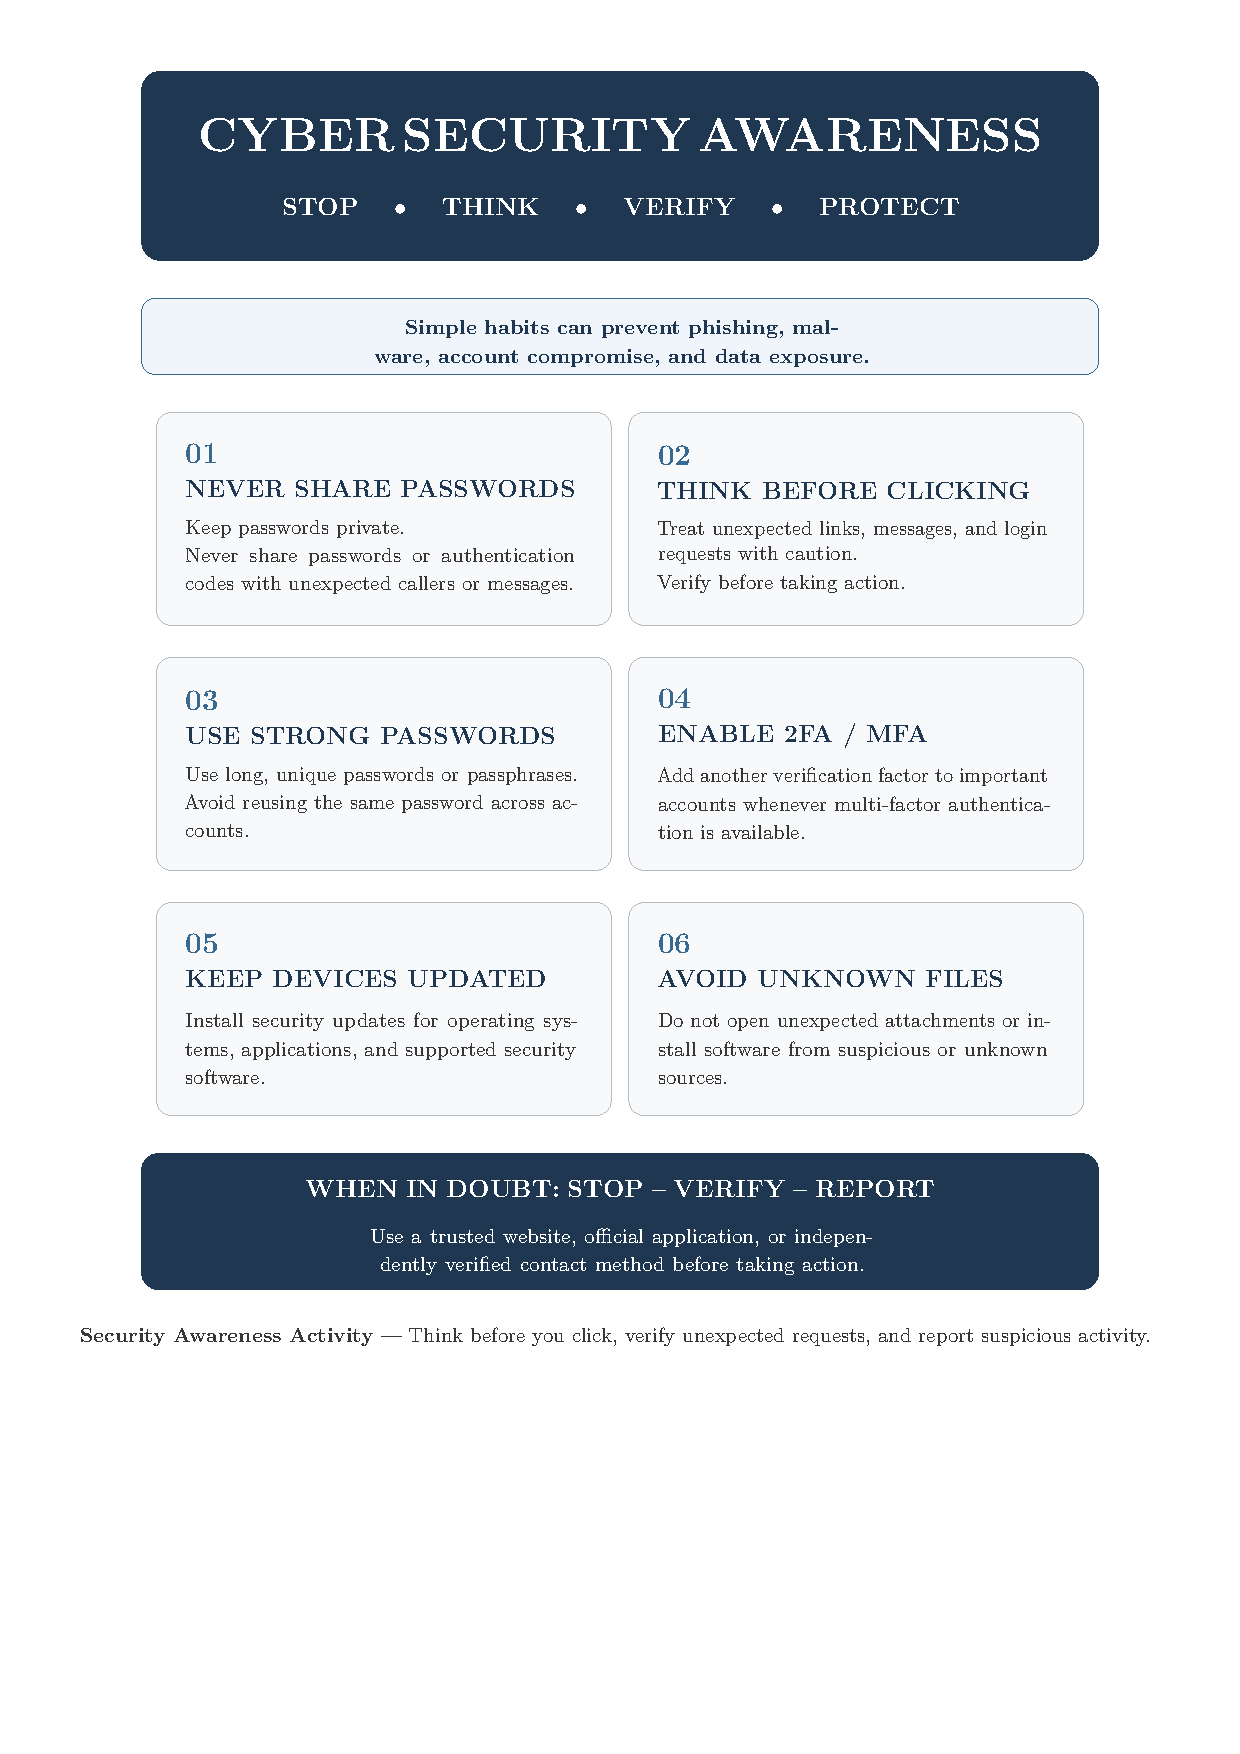
\includegraphics[width=0.82\textwidth]{images/cyber_security_awareness_poster.pdf}
\caption{Cyber Security Awareness Poster}
\end{figure}

\subsection{Poster Safety Tips}

\begin{enumerate}
    \item \textbf{Do not share passwords:} Passwords and authentication codes should remain private.
    \item \textbf{Be cautious with suspicious links:} Verify unexpected messages before clicking links.
    \item \textbf{Use strong passwords:} Use unique passwords or passphrases for important accounts.
    \item \textbf{Enable 2FA/MFA:} Use an additional authentication factor whenever the service supports it.
    \item \textbf{Install updates:} Security updates help address known vulnerabilities in software and operating systems.
    \item \textbf{Avoid unknown files:} Do not open unexpected attachments or install software from suspicious sources.
\end{enumerate}

\subsection{Why These Tips Matter}

Security awareness is a preventive layer that helps users recognize and avoid unsafe actions. Password protection reduces credential exposure, MFA adds an additional authentication layer, updates reduce exposure to known vulnerabilities, and careful handling of links and files reduces common phishing and malware delivery paths.

\subsection{Suggested Awareness Activity}

The poster can be shared in a classroom, internship group, lab environment, or internal awareness channel. A participant can then be asked to identify which poster tip applies to a short security scenario, such as receiving an unexpected password-reset email, a suspicious attachment, or an unknown software installer.

\textbf{Safety Note:} The activity should use fictional or educational examples. It should not collect real passwords, OTPs, personal information, or credentials.

\subsection{Cybersecurity Connection}

Security awareness supports the human side of cybersecurity. Technical controls such as email filtering, endpoint protection, MFA, firewalls, and patch management are more effective when users also understand why safe behavior is required. Awareness activities therefore help connect individual actions with broader preventive and incident-response controls.

\subsection{Quick Check}

\begin{enumerate}
    \item Why should passwords never be shared with another person?
    \item What should you do before clicking an unexpected link?
    \item What additional protection does MFA provide?
    \item Why should operating systems and applications be updated?
    \item Why should unknown attachments and files be treated cautiously?
\end{enumerate}

\textbf{Answers}
\begin{enumerate}
    \item Sharing passwords can expose accounts to unauthorized access and removes control over the credential.
    \item Verify the message and destination independently before interacting with the link.
    \item MFA provides an additional authentication factor beyond the password.
    \item Updates can address known security vulnerabilities and improve security protections.
    \item They may contain malicious content or lead to malware infection or other compromise.
\end{enumerate}

\subsection{Task 6 Summary}

The awareness poster communicates six practical security habits: keep passwords private, think before clicking, use strong passwords, enable MFA, keep devices updated, and avoid unknown files. These simple actions can reduce common phishing, malware, and account-compromise risks and can be reinforced through regular security-awareness activities.

\subsection{Documentation References}

\begin{enumerate}
    \item CISA -- Secure Our World and phishing-awareness guidance.
    \item FTC Consumer Advice -- phishing and scam-awareness guidance.
    \item NIST -- Phishing guidance and phishing-awareness examples.
    \item NIST Cybersecurity Framework 2.0.
\end{enumerate}

\end{document}
